\section{Part 2 - Dataset Analysis}

In this section we show the details and results of our dataset analysis and how it relates
to our research objectives discussed in Part 1.

\subsection{Dataset demographics}

In "Sub-objective 1", we explained why understanding the dataset demographics is essential to ensure
our prediction model does not suffer from any biases.

We start by counting the number of patients with and without reported heart disease. Table \ref{demographics-target-percent}
shows the percentage of patients with and without heart disease. Figure \ref{demographics-target-count} shows
the total number of patients with and without a heart condition.

\small
\begin{tabularx}{\linewidth}{ | X | X |}
    \caption{Distribution of patients with and without a heart condition}\label{demographics-target-percent} \\
    \hline
    \textbf{Target} & \textbf{Count}\\
    \hline
    No heart disease & 42\% \\
    \hline
    Heart disease & 58\% \\
    \hline
\end{tabularx}
\normalsize

\begin{figure}
    \caption{Number of patients with and without a heart condition}\label{demographics-target-count}
    \centering
    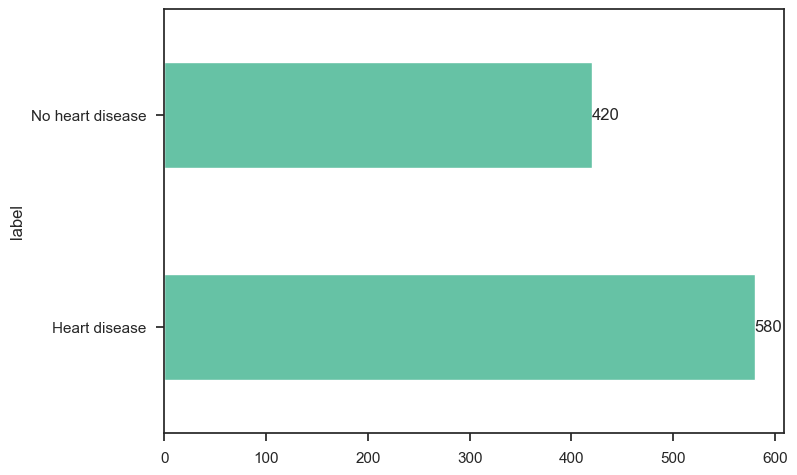
\includegraphics[width=\linewidth]{media/demographics-01-target.png}
\end{figure}

These values show that the dataset \textbf{is well balanced between assigned labels} (i.e. classification). This
is important to ensure that our prediction model has enough training data.

\subsubsection{Gender demographics}

To identify potential gender bias and ensure that our prediction model is accurate for any gender, we analyse
the distribution of data across genders.

Figure \ref{demographics-gender-target-count} shows that there are more than double the amount of male patients
compare to female patients. Table \ref{demographics-gender-percent} shows that the number of female patients is
only 23\% of the total. This \textbf{could point to a lower incidence of heart-related conditions in the female population},
but we cannot confirm it without gathering more details about the recruitment strategy for the dataset.
    
\begin{figure}
    \caption{Number of patients of each gender grouped by class}\label{demographics-gender-target-count}
    \centering
    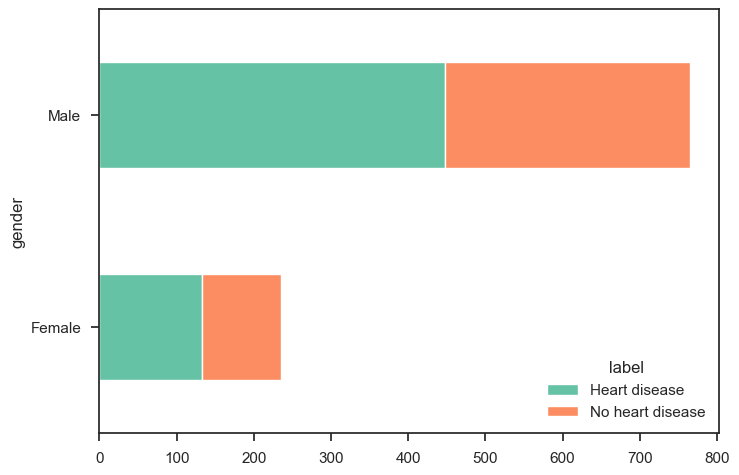
\includegraphics[width=\linewidth]{media/demographics-03-gender-target-count.png}
\end{figure}

\small
\begin{tabularx}{\linewidth}{ | X | X |}
    \caption{Distribution of patients of each gender}\label{demographics-gender-percent} \\
    \hline
    \textbf{Gender} & \textbf{Percentage}\\
    \hline
    Female & 23\% \\
    \hline
    Male & 77\% \\
    \hline
\end{tabularx}
\normalsize

Assuming that the bias towards male patients is not representative of disease incidence, we must at least
ensure that the distribution of patients with disease is constant across genders, so that the prediction
model will not tend to disproportionally apply a specific class to a whole gender.

Figure \ref{demographics-gender-target-percent} shows the distribution of patients with disease across genders,
and confirms that indeed the distribution is balanced.

\begin{figure}
    \caption{Distribution of patients of each gender grouped by class}\label{demographics-gender-target-percent}
    \centering
    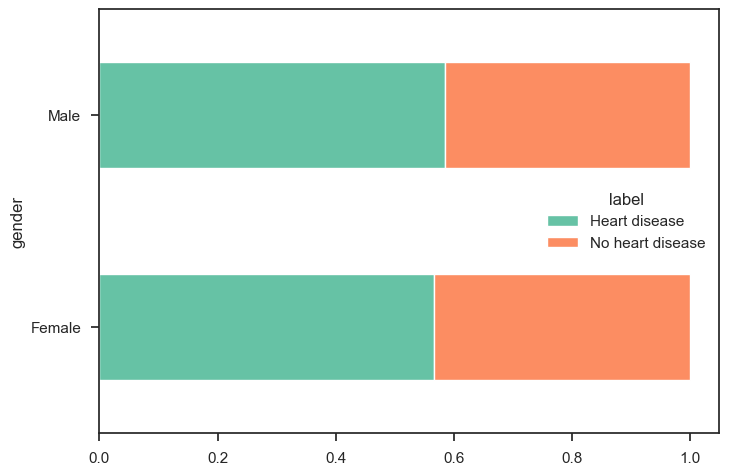
\includegraphics[width=\linewidth]{media/demographics-04-gender-target-percentage.png}
\end{figure}


\begin{figure}
    \caption{Distribution of genders across age groups}\label{demographics-gender-agegroup-count}
    \centering
    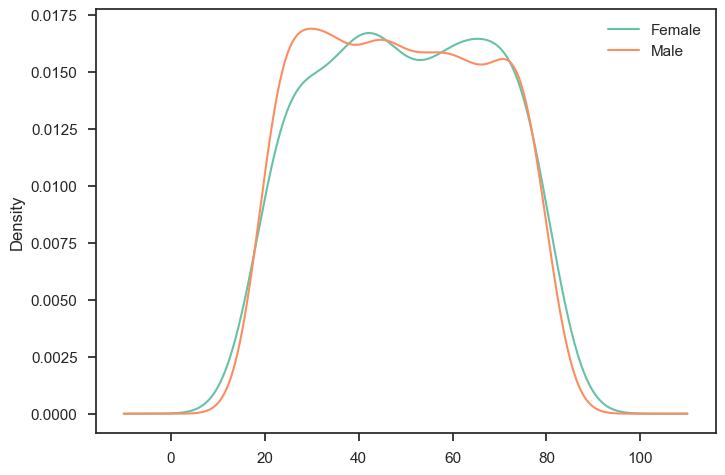
\includegraphics[width=\linewidth]{media/demographics-02-gender-age.png}
\end{figure}

\subsubsection{Age demographics}

\begin{figure}
    \caption{Distribution of patients of each age group grouped by class}\label{demographics-agegroup-target-percent}
    \centering
    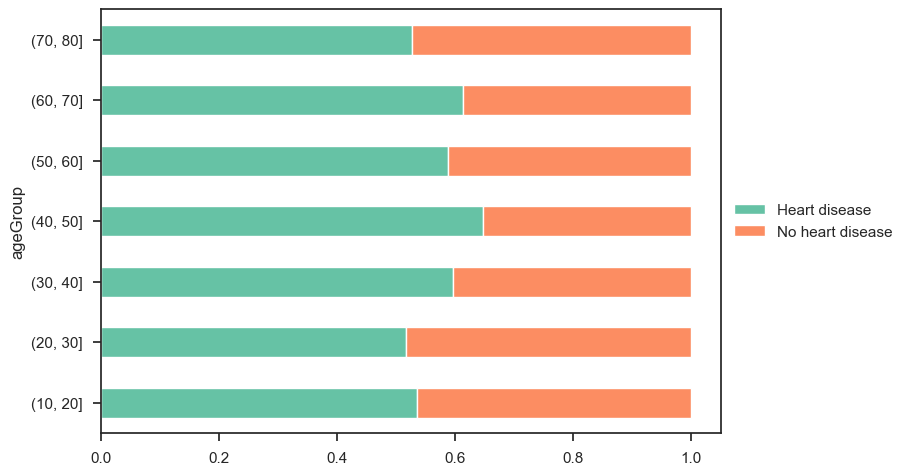
\includegraphics[width=\linewidth]{media/demographics-05-agegroup-target-percentage.png}
\end{figure}



\subsection{Frequency Analysis}

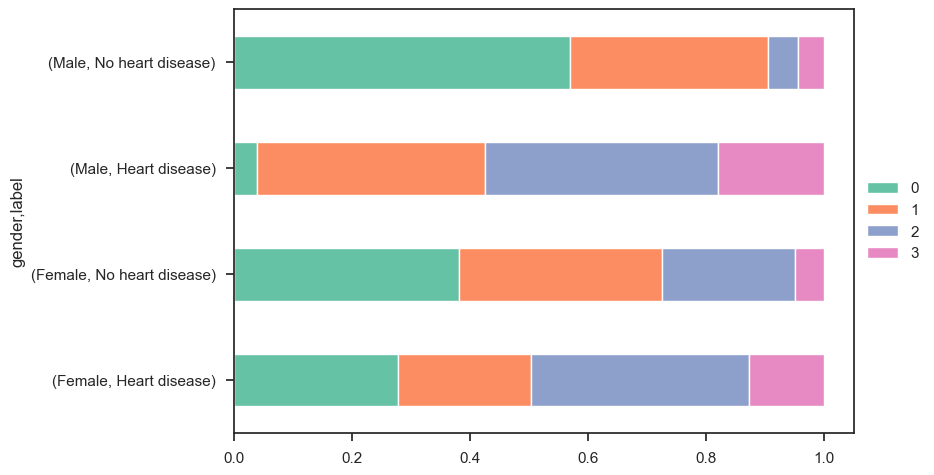
\includegraphics[width=0.8\linewidth]{media/frequency-01-gender-vessels.png}

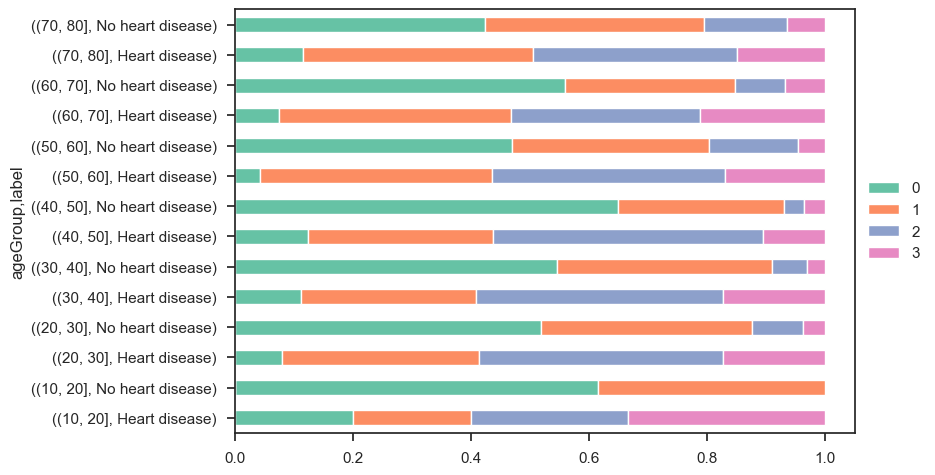
\includegraphics[width=0.8\linewidth]{media/frequency-02-agegroup-vessels.png}

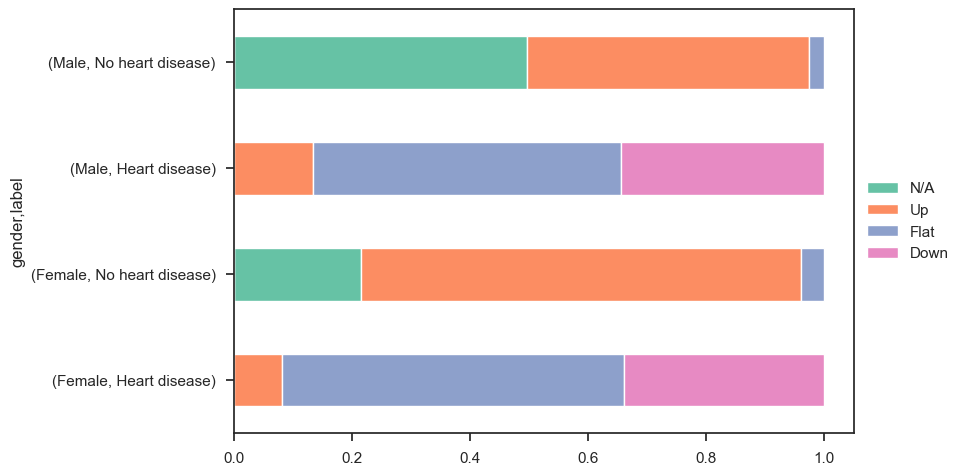
\includegraphics[width=0.8\linewidth]{media/frequency-03-gender-slope.png}

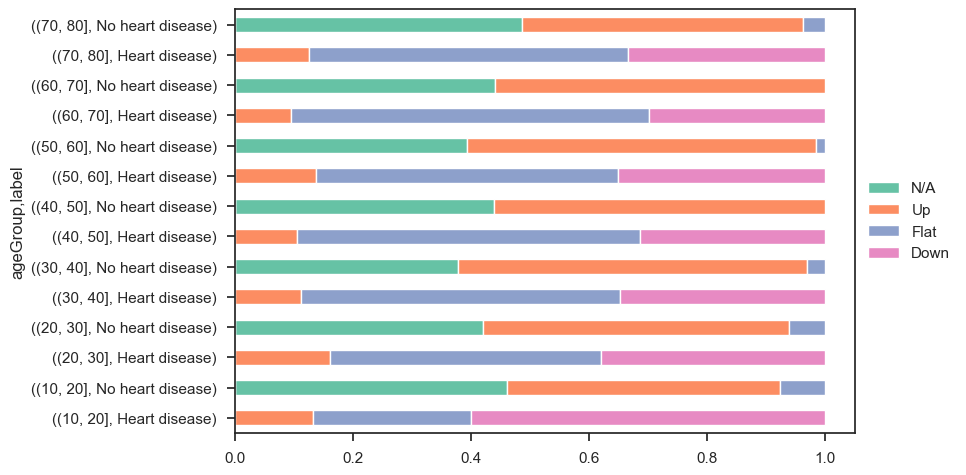
\includegraphics[width=0.8\linewidth]{media/frequency-04-agegroup-slope.png}

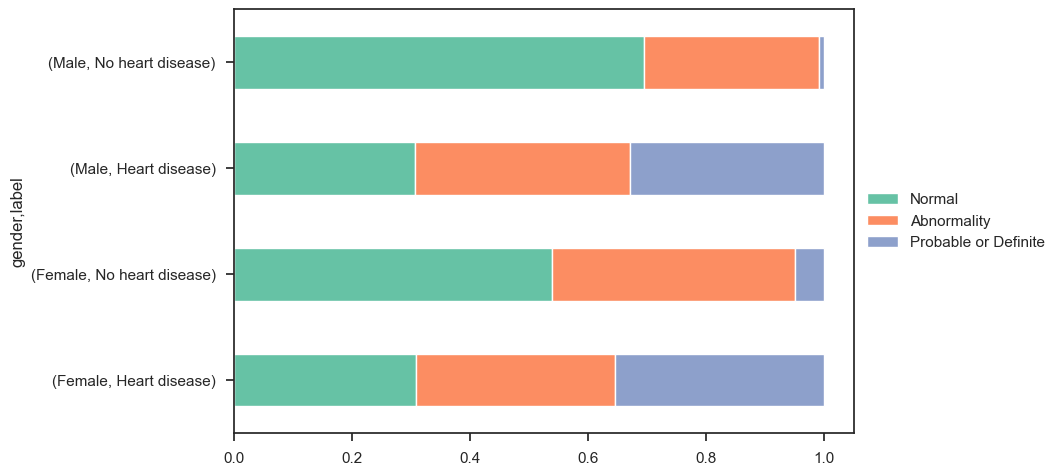
\includegraphics[width=0.8\linewidth]{media/frequency-05-gender-ecg.png}

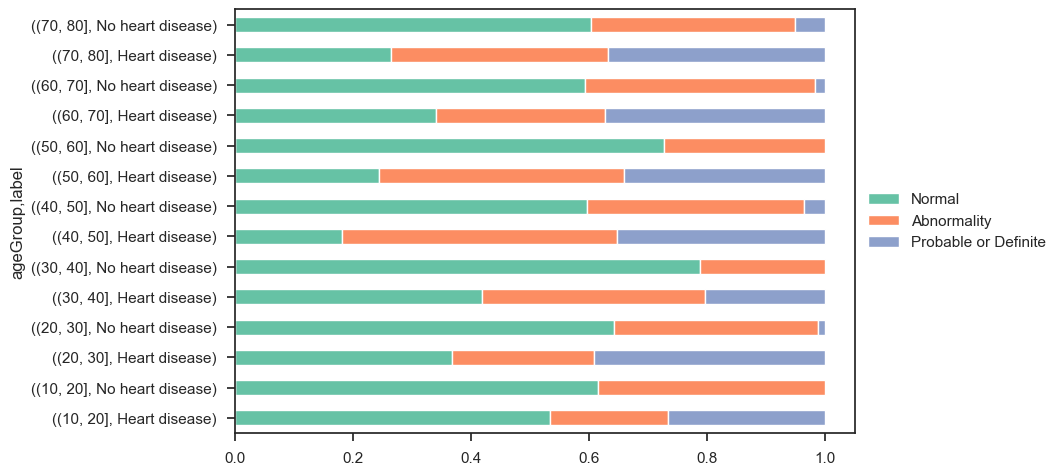
\includegraphics[width=0.8\linewidth]{media/frequency-06-agegroup-ecg.png}

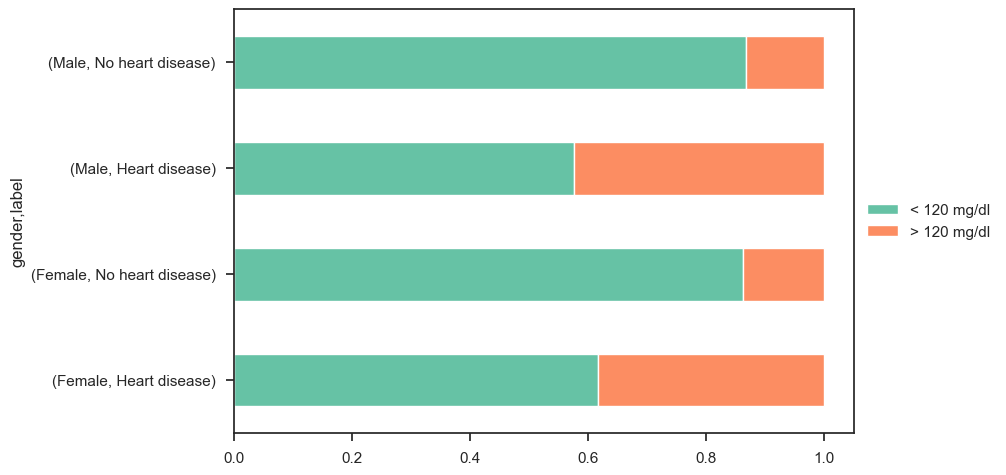
\includegraphics[width=0.8\linewidth]{media/frequency-07-gender-bloodsugar.png}

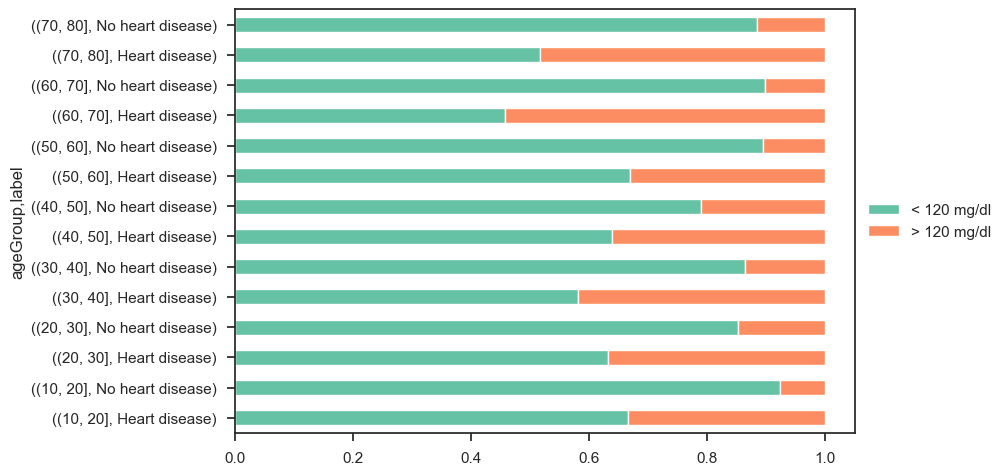
\includegraphics[width=0.8\linewidth]{media/frequency-08-agegroup-bloodsugar.png}

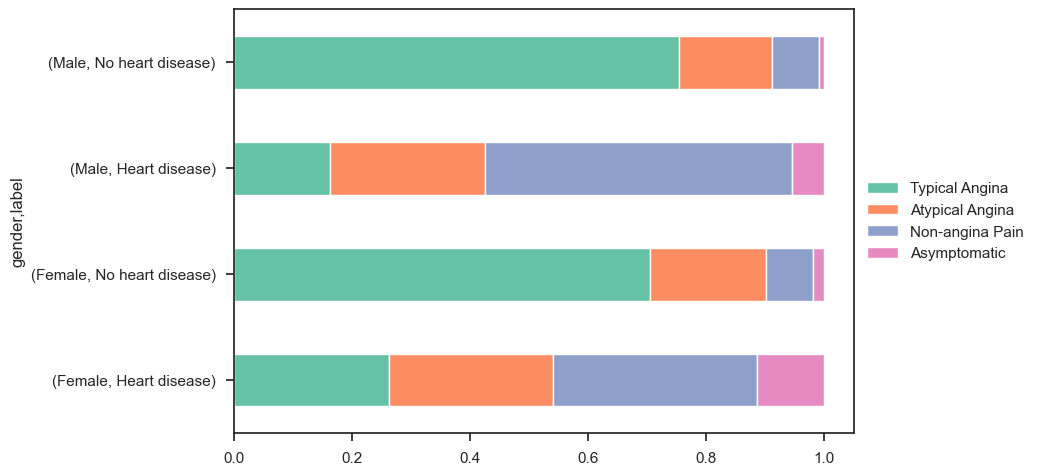
\includegraphics[width=0.8\linewidth]{media/frequency-09-gender-paintype.png}

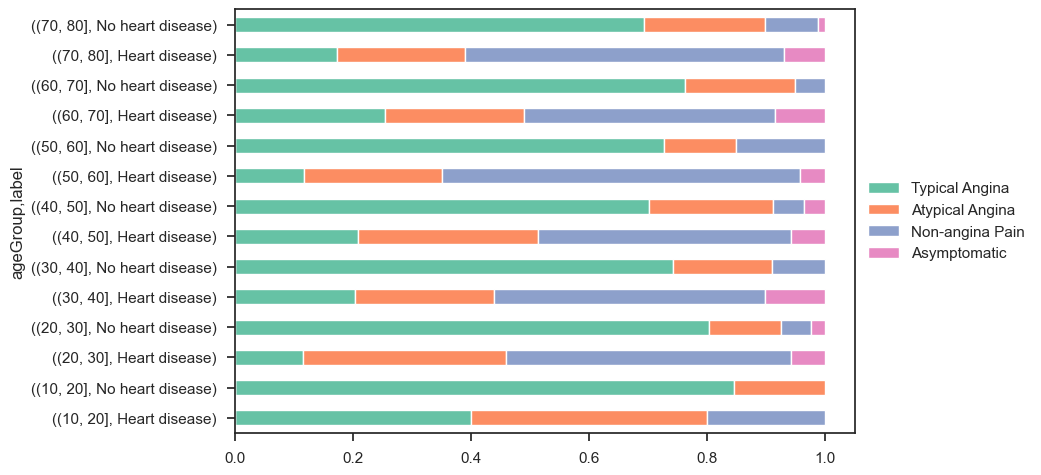
\includegraphics[width=0.8\linewidth]{media/frequency-10-agegroup-paintype.png}

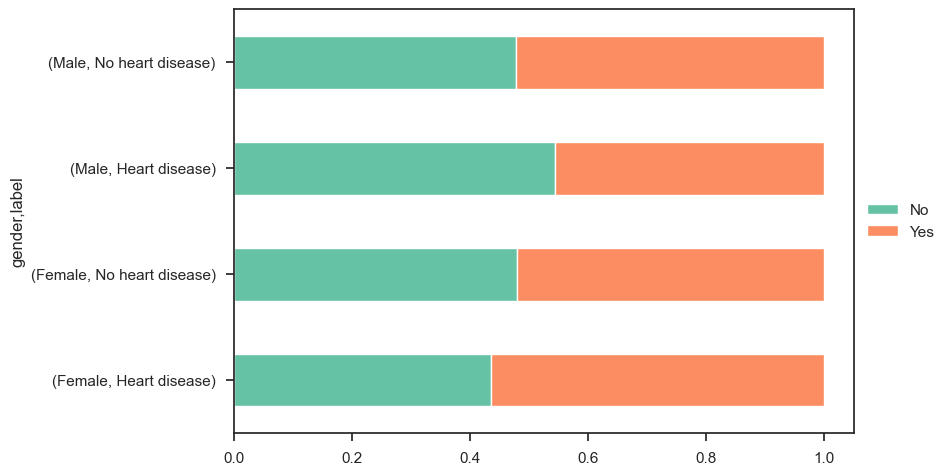
\includegraphics[width=0.8\linewidth]{media/frequency-11-gender-exerciseangina.png}

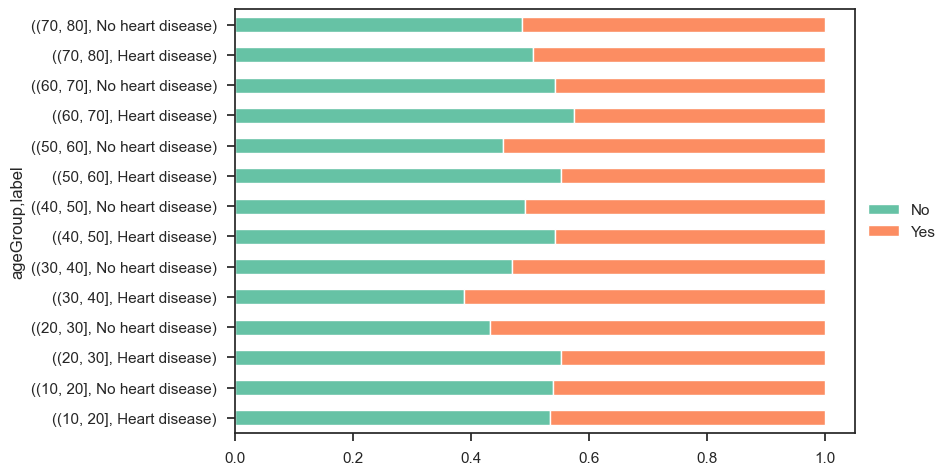
\includegraphics[width=0.8\linewidth]{media/frequency-12-agegroup-exerciseangina.png}

\subsection{Data spread and variability}


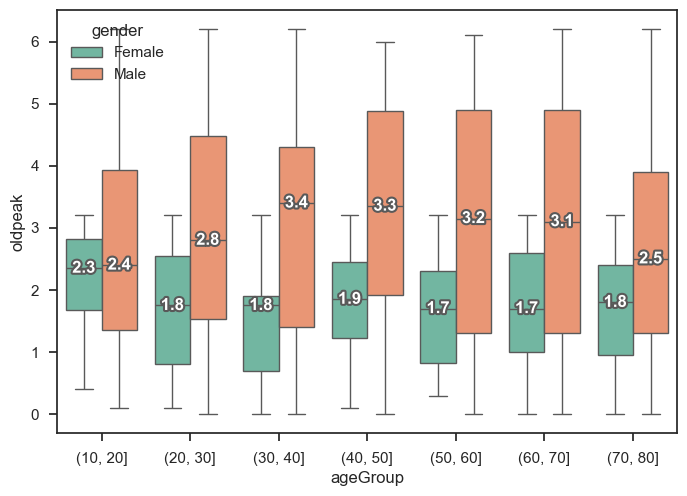
\includegraphics[width=0.8\linewidth]{media/boxplot-01-agegroup-gender-oldpeak.png}

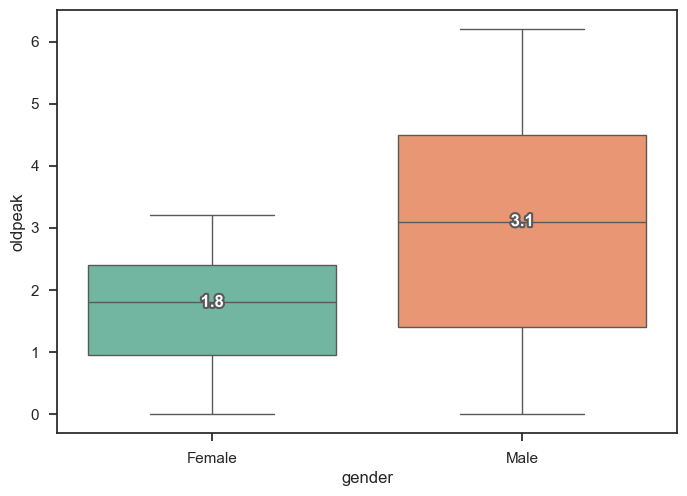
\includegraphics[width=0.8\linewidth]{media/boxplot-02-gender-oldpeak.png}

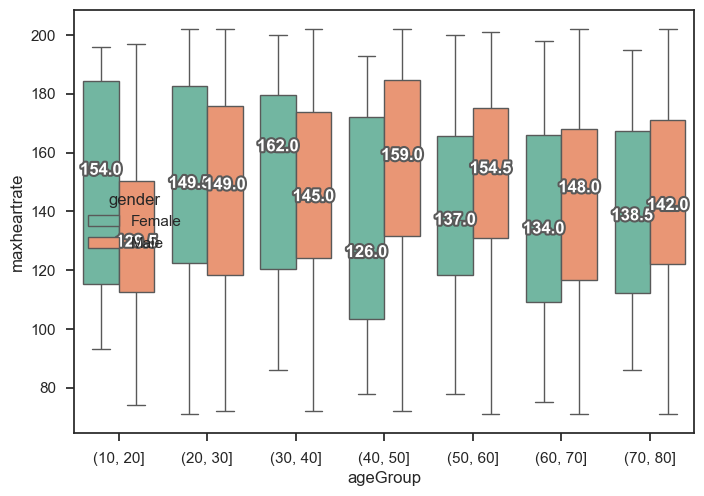
\includegraphics[width=0.8\linewidth]{media/boxplot-03-agegroup-gender-heartrate.png}

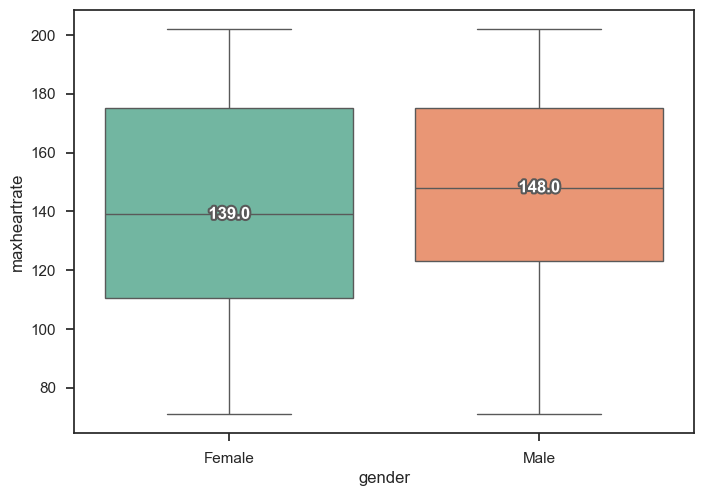
\includegraphics[width=0.8\linewidth]{media/boxplot-04-gender-heartrate.png}

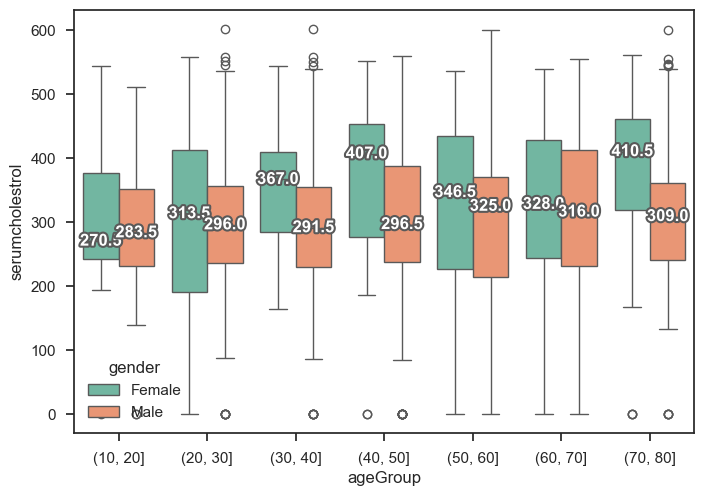
\includegraphics[width=0.8\linewidth]{media/boxplot-05-agegroup-gender-cholesterol.png}

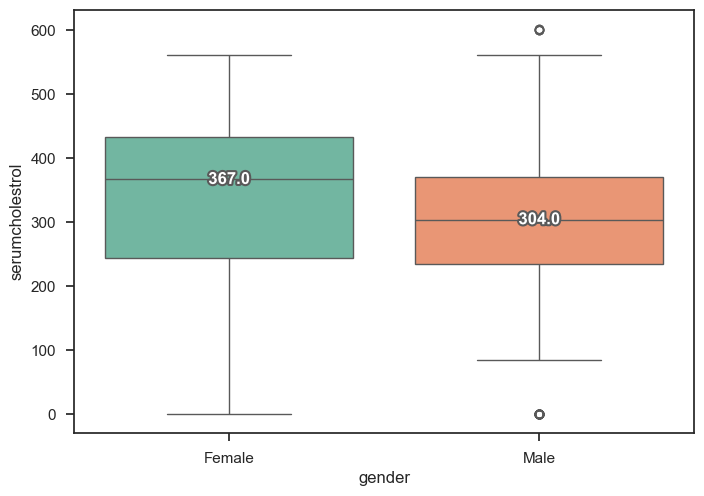
\includegraphics[width=0.8\linewidth]{media/boxplot-06-gender-cholesterol.png}

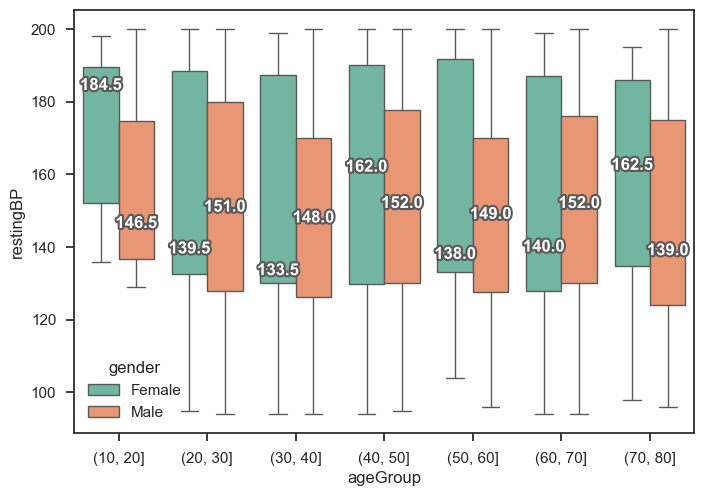
\includegraphics[width=0.8\linewidth]{media/boxplot-07-agegroup-gender-bp.png}

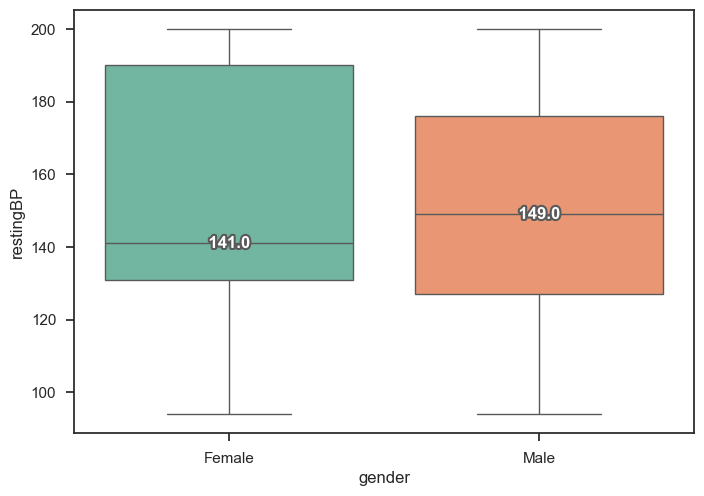
\includegraphics[width=0.8\linewidth]{media/boxplot-08-gender-bp.png}

\subsection{Correlation analysis}

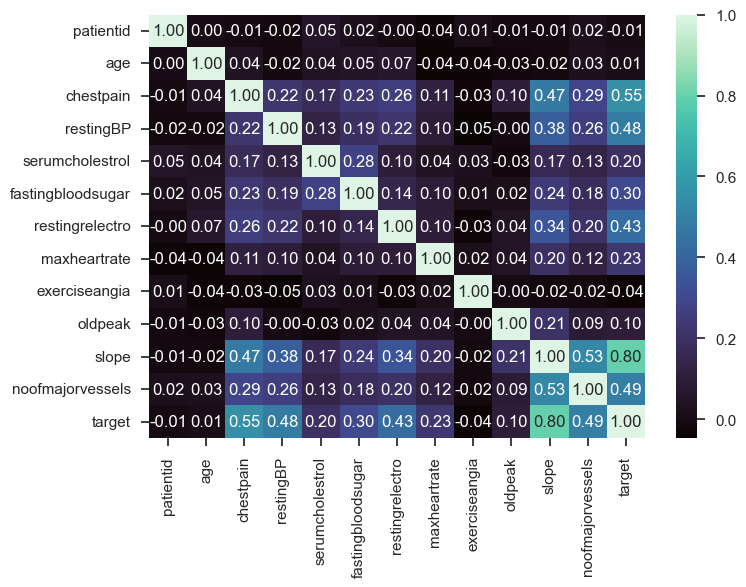
\includegraphics[width=0.8\linewidth]{media/correlation-matrix.png}